\documentclass{beamer}
\usepackage[utf8]{inputenc}
\usetheme{Copenhagen}
\usecolortheme{default}

\usepackage{graphicx}
\graphicspath{ {../Resources/} }

\usepackage{listings}

\title{An Introduction to Git and GitHub}
\author{Lan Peng}
\institute{Department of Industrial and Systems Engineering, University at Buffalo, SUNY}
\date{\today}

\begin{document}
	\frame{\titlepage}
	
	\begin{frame}
		\frametitle{Outline}
		\tableofcontents
	\end{frame}

	\section{Version control and Git}
		\subsection{Version control}
			\begin{frame}
				\frametitle{Version Control}
				\begin{align}
					\centering
					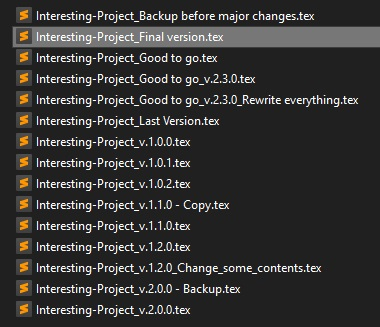
\includegraphics[height=5cm]{version_control} \nonumber
				\end{align}			
			\end{frame}

			\begin{frame}
				\frametitle{Version Control}
				The disadvantage of control version in this way
				\begin{itemize}
					\item Too messy, hard to find the latest (time stamps sometimes can't help)
					\item Cannot compare the difference between each version
					\item Cannot merge changes in different edition from one or more participants
					\item Cannot keep track of changes
				\end{itemize}
			\end{frame}
		\subsection{Git}
			\begin{frame}
				Git is a distributed version-control system for tracking changes in source code during software development.It is designed for coordinating work among programmers, but it can be used to track changes in any set of files.
				\begin{align}
					\centering
					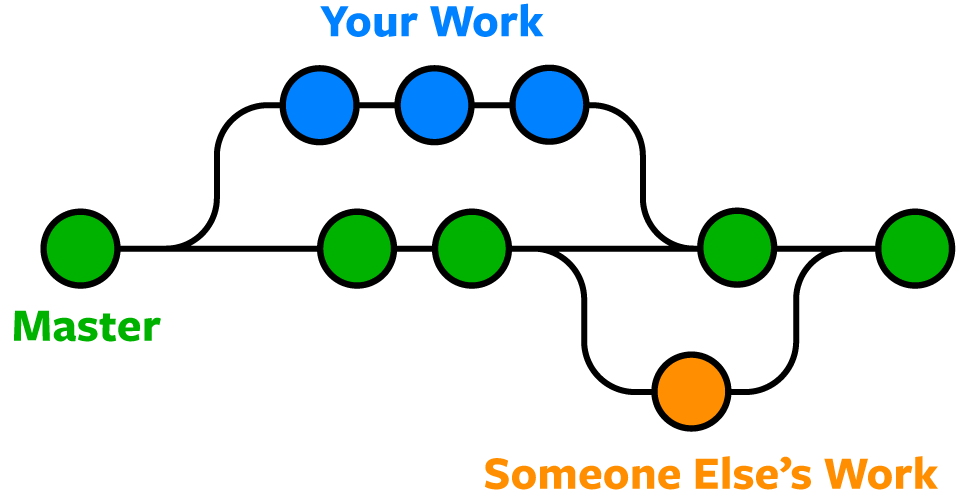
\includegraphics[height=4cm]{git-branches-merge} \nonumber
				\end{align}
			\end{frame}

	\section{Git and GitHub}
		\subsection{Installation Git}
			\begin{frame}
				\frametitle{Installation}
				\begin{itemize}
					\item Windows: \url{https://git-scm.com/downloads}
					\item Linux: \texttt{sudo apt-get install git}
					\item Mac OS: 
						\begin{enumerate}
							\item Install \texttt{Xcode} from AppStore 
							\item Run \texttt{Xcode} 
							\item In \texttt{Xcode -> Preferences} find \texttt{Downloads} 
							\item Choose \texttt{Command Line Tools}, install it
						\end{enumerate}					
				\end{itemize}
			\end{frame}

			\begin{frame}
				\frametitle{Installation}
				After installation, open the terminal and input \texttt{git} to see if it is successfully installed. There should be something like this:
				\begin{align}
					\centering
					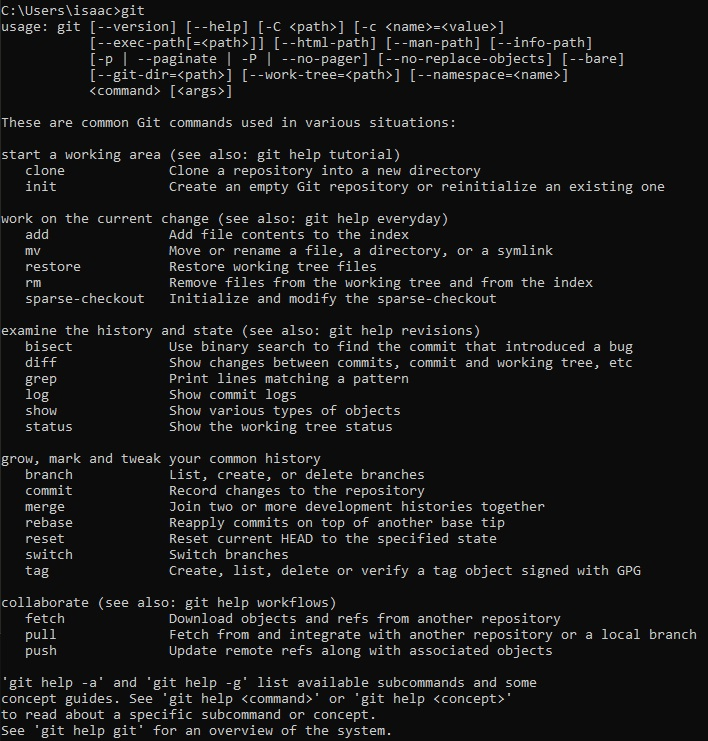
\includegraphics[height=5cm]{git_installed} \nonumber
				\end{align}
			\end{frame}

		\subsection{What is GitHub}
			\begin{frame}
				\frametitle{GitHub}
				\begin{itemize}
					\item A/the global company that provides hosting for software development version control using Git
					\item A website Microsoft just bought for \$7.5 billion dollar
					\item A website that you can goof around when you are bored at coding and don't need to worry about getting caught by your manager (she/he might be doing the same thing)
				\end{itemize}
			\end{frame}

	\section{Using Git and GitHub}
		\subsection{Initialize/Clone}
			\begin{frame}
				\frametitle{Initialize/Clone}
				\begin{itemize}
					\item \texttt{git init}
				\end{itemize}
				Create a \texttt{.git} folder in current path, making current path a git repository

				\begin{itemize}
					\item \texttt{git clone}
				\end{itemize}
				From a remote repository clone to current path
			\end{frame}

		\subsection{Branch}
			\begin{frame}
				\frametitle{Branch}
				\begin{itemize}
					\item List branches\\
						\texttt{git branch}
					\item Create a new branch\\
						\texttt{git branch [branchName]}
					\item Switch between branches\\
						\texttt{git checkout [branchName]}
					\item Create and switch to branch (2 steps in 1 line)\\
						\texttt{git checkout -b [branchName]}
				\end{itemize}
			\end{frame}

			\begin{frame}
				\frametitle{Branch (cont.)}
				\begin{itemize}						
					\item Delete a branch (won't delete if there are unmerged changes)\\
						\texttt{git branch -d [branchName]}
					\item Delete a branch (will delete even if branch has unmerged changes)\\
						\texttt{git branch -D [branchName]}
					\item Rename a branch, default to be current branch\\
						\texttt{git branch -m [oldBranchName] [newBranchName]}
					\item Back to main branch\\
						\texttt{git checkout master}
				\end{itemize}
			\end{frame}

		\subsection{Commit}
			\begin{frame}
				\frametitle{Commit}
				The following are steps for commit
				\begin{itemize}
					\item Step 0: Check changes using \texttt{git status}
					\item Step 1.1: Add changes by \texttt{git add <filename>} or add all changes by \texttt{git add -A}
					\item Step 1.2: Discard changes by \texttt{git checkout <filename>}
					\item Step 2: Commit the changes by \texttt{git commit -m "Some description"}
				\end{itemize}
				After commit, the next step is push it to remote.

				If you don't want to commit to remote and wnt to undo it
				\begin{itemize}
					\item Step 1: Find commit hash, \texttt{git log}
					\item Step 2: Revert commit, \texttt{git revert [commitHash]}, it actually create a new commit to revert this commit
				\end{itemize}
			\end{frame}

		\subsection{Pull/push}
			\begin{frame}
				\begin{itemize}
					\item \texttt{git fetch}
				\end{itemize}
				Check if there is a new version, you might not want to pull at this moment

				\begin{itemize}
					\item \texttt{git pull origin <branch>}
				\end{itemize}
				From remote pull changes into local

				\begin{itemize}
					\item \texttt{git push origin <branch>}
				\end{itemize}
				Sync remote repository with local repository

				\begin{alertblock}{Important}
					Always remember to pull before start editing, otherwise you might have conflicts
				\end{alertblock}
			\end{frame}

		\subsection{Merge, Pull request}
			\begin{frame}
				\frametitle{Merge}
				\begin{itemize}
					\item Step 1. Go to the branch you need to merge into (e.g. master)
					\item Step 2. \texttt{git merge <branch>}
				\end{itemize}
			\end{frame}

			\begin{frame}
				\frametitle{Pull Request}
				On GitHub website, you can find a buttom named \texttt{New pull request}. It ``requests'' the owner/admin of the repository to do a ``pull'' from your branch. After the owner pull your branch, your branch in remote will be deleted, but you will still have your local copy so the workflow will not be affected.
			\end{frame}

		\subsection{Conflict}
			\begin{frame}
				\frametitle{Conflict}
				If your version is behind the remote version, i.e., someone had changed the files and push to remote repository, you also made some changes in the same file before you \texttt{git pull} from remote. Then when you try to \texttt{git push} your version to remote, a message will alert to let you \texttt{git pull} first.

				Git will try to solve the conflict by itself, but it might not work. Then you need to solve the conflict.
			\end{frame}

			\begin{frame}
				\frametitle{Solve conflict}
				If the conflict happens in a non-binary file (e.g., \texttt{.py}, \texttt{.tex}, basic every file can be edited by text editor), it is easy to solve:

				Use text editor to open the conflict file, search for the following structure:
				\begin{align}
					\centering
					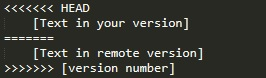
\includegraphics{conflict} \nonumber
				\end{align}
				Edit it and \texttt{git add}, \texttt{git commit} again
			\end{frame}

			\begin{frame}
				For binary files (e.g., \texttt{.pdf}, \texttt{.exe}, \texttt{.docx}, \texttt{.dll}), it is hard to merge them. What we can do is choose a version.
				\begin{itemize}
					\item Resolve using your version\\
						\texttt{git add [conflictFileName]}\\
						\texttt{git commit -m "I used mine version"}
					\item Resolve using remote version\\
						\texttt{git checkout [conflictFileName]}\\
						\texttt{git add [conflictFileName]}\\
						\texttt{git commit -m "I used their version"}
				\end{itemize}
			\end{frame}

			\begin{frame}
				\frametitle{Tip}
				We don't like to merge changes in the same file, here are some tips to avoid that:
				\begin{itemize}
					\item Design by module, break large files into smaller files. Each group member works on separated file, have someone (e.g., team leader) design the interface between modules
					\item Sync with master branch more often
					\item Commit with small changes (it depends)
				\end{itemize}
			\end{frame}
		\subsection{Revert/Reset}

		\subsection{Others}
			Your can try some other commands... just for fun
			\begin{itemize}
				\item \texttt{git diff}
				\item \texttt{git log}
			\end{itemize}

\end{document}